

\documentclass[a4paper]{article}

\usepackage{amsmath}
\usepackage{hyperref}
\usepackage{biblatex}
\usepackage{enumerate}
\usepackage{graphicx}
\usepackage{stmaryrd}
\usepackage[dvipsnames]{xcolor}
\usepackage{listings}


\addbibresource{refs.bib}

\begin{document}

\author{Ola Bratt \\
  \href{mailto:ola.bratt@gmail.com}{ola.bratt@gmail.com}
  \and
  Patrick Attimont \\
  \href{patrickattimont@gmail.com}{patrickattimont@gmail.com}
}

\title{DAT565/DIT407 Assignment 1}
\date{2024-01-16}

\maketitle

This paper is addressing the assignment 1 study queries within the \emph{Introduction to Data Science \& AI}, DIT407 course at 
the University of Gothenburg. The main source of information for this project
is derived from the lectures and Skiena~\cite{Skiena:2024}. Assignment 1 focuses on using Python tools, such as Pandas, NumPy, and Matplotlib. 

\section*{Problem 1: Dependency Ratio}

In Figure~\ref{fig:ratio} the Dependecy Ratio of Sweden from 1860 to 2022 is show.
The ratio is calculated by using the data from SCB~\cite{SCB:2023}. The ratio is calculated by dividing 
the total dependent population (children, 0-14 years  and elderly, 65+) with the labor force, 15-64 years and multiply with 100 (Equation~\ref{equation:dependencyratio}).


\begin{equation}
  \label{equation:dependencyratio}
  Dependency \thinspace ratio = 100 * \cfrac{ children + elderly}{labor \thinspace force}
\end{equation}

\begin{figure}[h]
  \begin{center}
    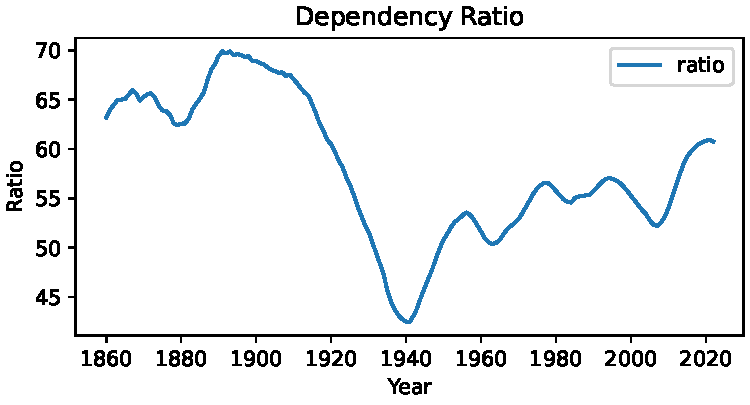
\includegraphics[width=\textwidth]{ratio.pdf}
    \caption{Dependecy ratio}
    \label{fig:ratio}
  \end{center}
\end{figure}

\newpage

In Figure~\ref{fig:fractions} the diffrent fractions of the population is shown. The fractions 
are calculated by dividing the population group (children, elderly and total depentent population) with the total population. 
The fractions are calculated by using the data from SCB~\cite{SCB:2023}.


\begin{figure}[h]
  \begin{center}
    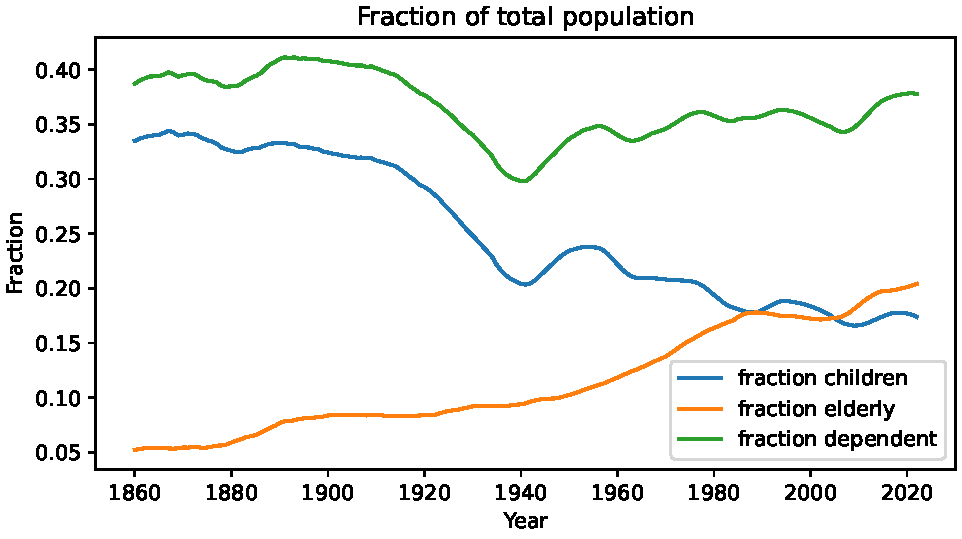
\includegraphics[width=\textwidth]{fractions.pdf}
    \caption{Fractions}
    \label{fig:fractions}
  \end{center}
\end{figure}


\section*{Conclusions}
Advances in healthcare, improved living conditions, and better access to medical services have contributed to increased life 
expectancy in Sweden. Longer lifespans result in a larger proportion of the population falling into the elderly category,
leading to a shift in the age distribution. This is evident in Figure~\ref{fig:fractions}, where the fraction of the elderly consistently increases over the entire time span.

Simultaneously, there is a noticeable declining trend in the fraction of children. This phenomenon is attributed to the decreasing fertility rate in Sweden since the 1960s. 
Various factors contribute to this decline, including postponed marriage, heightened focus on education and career pursuits among women, and evolving societal norms.

Furthermore, a distinct dip in the fraction of children is observed around 1940, likely attributable to the impact of the Second World War.

Many industrialized countries share common demographic challenges, such as aging populations, low fertility rates, and the need for immigration to offset demographic imbalances, Eurostat~\cite{Eurostat:2023}. 
These trends have implications for social welfare systems, healthcare, and economic sustainability. 

\newpage

\printbibliography

\section*{Appendix: Source Code}

\lstset{
  language=Python,
  basicstyle=\ttfamily,
  commentstyle=\color{OliveGreen},
  keywordstyle=\bfseries\color{Magenta},
  stringstyle=\color{YellowOrange},
  numbers=left,
  basicstyle=\footnotesize,
  breaklines=true,
  postbreak=\mbox{\textcolor{red}{$\hookrightarrow$}\space}
}


\lstinputlisting{assignment1.py}

\end{document}
